%TODO opisać VLBI, laser ranging, coordinates like ITRF :)\\
%TODO trzeba opisać pokrutce aktualne systemy satelitarne GPS, GALILEO, GLONASS, BaiDou-Compass, indian IRNSS\\
%TODO trzeba opisać na czym polega RTK, DGPS etc.

W tym rozdziale omówione zostały podstawy teoretyczne dotyczące infrastruktury geodezyjnej niezbędnej do określania 
położenia punktów a zatem i obiektów w przestrzeni. Na początku zostały omówione zagadnienia dotyczące geodezji kosmicznej,
której techniki zrewolucjonizowały możliwości człowieka w dziedzinie nawigacji tak bardzo istotnej dla rolnictwa precyzyjnego.
W dalszej części rozdziału opisano pokrótce algorytmy wyznaczania pozycji w nawigacji satelitarnej oraz inercjalnej, a tekże metodę 
integracji tych dwóch jakże uzupełniających się technik. 

\section{Układ Odniesienia}
Przykładem obrazującym potrzebę posiadania stabilnego w czasie i przestrzeni układu odniesienia są ścieżki przejazdowe,
dzięki którym koła pojazdu nie niszczą upraw. Aby możliwe było tworzenie ścieżek przejazdowych dokładność pozycjonowania 
traktora bądź innego narzędzia musi być rzędu kilku centymetrów względem poprzednich przejazdów. Jedynym sposobem 
na uzyskanie wyżej wymienionej dokładności prowadzenia maszyn jest dysponowanie precyzyjnie zdefiniowanym 
układem, w którym przechowywane będą współrzędne poprzednich przejazdów i w którym będzie dostarczana pozycja w 
czasie rzeczywistym. Ponieważ dokładność wyznaczenia pozycji w danym układzie zależy od dokładności realizacji tego układu,
w praktyce przyjmuje się, że układ odniesienia powinien być zrealizowany o rząd wielkości dokładniej niż wymagana dokładność pozycjonowania. \cite[][strona 210]{ggos}
Poniżej opisano dwa najważniejsze systemy odniesień przestrzennych oraz ich realizacje.
	\subsection{ICRS}
International Celestial Reference System - Międzynarodowy Niebieski System Odniesienia realizowany poprzez technikę VLBI - interferometria długich baz, 
składa się z zestawu procedur i konwencji oraz odpowiednich zasad modelowania koniecznych do zdefiniowania w dowolnym momencie czasu trzech osi kartezjańskiego 
układu współrzędnych w przestrzeni kosmicznej \cite{IERS_ICRS}. Osie tego układu są zdefiniowane w taki sposób aby ich kierunki wzgledem najodleglejszych obiektów 
kosmosu były stałe. Z punktu widzenia kinematyki system jest quasi-inercjalny \cite[][strona 23]{KRYNSKI_SYSTEMY}.
System jest zrealizowany fizycznie za pomocą układu odniesienia ICRF - International Celestial Reference Frame, który składa się z zbioru precyzyjnie
wyznaczonych współrzędnych pozagalaktycznych obiektów takich jak: kwazary oraz aktywne jądra niektórych galaktyk.
Ruchy własne powyższych radioźródeł są zaniedbywalne z punktu widzenia docelowej dokładności wyznaczania współrzędnych.\cite[][strona 21]{IERS_2010}.
Początek układu współrzędnych w systemie ICRS został zdefiniowany w punkcie barycentrum układu słonecznego. \cite[][strona 163]{BRZEZINSKI_2012}.
Profesorowie Brzeziński oraz Rogowski powiadają, że dokładność kierunku osi układu ICRF waha się w granicach 20 mikrosekund miary łukowej
(50 odpowiada 1.5 mm na pow. Ziemi), co przy dostępności 
precyzyjnego modelu precesji - nutacji pozwala stwierdzić, że ICRF jest najlepszym inercjalnym układem odniesienia dostępnym obecnie\cite[][strona 164]{BRZEZINSKI_2012}.
Warto zadać pytanie: dlaczego system ICRS wraz z jego realizacją w postaci ICRF są takie ważne z punktu widzenia rolnictwa precyzyjnego?
Według autorów pracy \cite[][strona 164]{BRZEZINSKI_2012} ponieważ z wystarczającą dokładnością możemy przyjać iż, układ ICRF jest inercjalny, 
są w nim zatem spełnione równania \ref{satellite_eq} ruchu sztucznych satelitów Ziemi wolne od tzw. pozornych sił bezwładności.
\begin{equation} \label{satellite_eq}
\quad \vec{ \ddot{r} } + \mu \frac{ \vec{r} } { \lvert { \vec{r} }^{\,3} \rvert } = \vec{a_p}
\end{equation} 
Gdzie $ \vec{r} $ oznacza pozycję satelity względem środka mas Ziemi.\\
$\vec{ddot{r}}$ oznacza drugą pochodną wektora względem czasu.\\
$\mu = GM $ oznacza ziemską stałą grawitacji.\\
$\vec{a_p}$ wyraża przyspieszenia perturbujące np. pochodzące od promieni słonecznych.
Według autorów opracowania \cite[]{BRZEZINSKI_2012} po uprzednim scałkowaniu równania różniczkowego \ref{satellite_eq}
otrzymujemy chwilową pozycję satelity w inercjalnym systemie ICRS. Jedną z fundamentalnych funkcji systemu ICRS 
jest zatem dostarczanie odniesienia podczas wyznaczeń orbit sztucznych satelitów Ziemi. Punkty aproksymujące dyskretnie orbitę satelity 
są transformowane do systemu ITRS (patrz następny paragraf) w którym to systemie są publikowane gotowe produkty IGS. ( orbity + parametry zegarów).
Powyższą transformację opisano np. w monografi \cite[][strona 43]{IERS_2010}. Transformacja jest realizowana w oparciu o ruchy bieguna niebieskiego,
model precesji oraz nutacji a także ruchy bieguna ziemskiego. Warto zwrócić uwagę na fakt znacznego pogorszenia dokładności opisanej transformacji,
gdy jest ona wykonywana w czasie rzeczywistym w zastosowaniach nawigacyjnych. Dla przykładu wpływ pływów skorupy ziemskiej daje efekt rzędu 
$\frac{+}{-}25 cm$ \cite[][strona 166]{BRZEZINSKI_2012}. W różnicowych algorytmach pozycjonowania (RTK, DGPS etc.) 
efekty takie nie mają wielkiego znaczenia, natomiast w pomiarach absolutnych (ppp) wymagane jest ich jak najlepsze modelowanie.
	%%%%%%%%%%%%%%%%%%%%%
	\subsection{ITRS}
	%%%%%%%%%%%%%%%%%%%%%%
Terrestial Reference System - Ziemski System Odniesienia jest to system odniesień przestrzennych wirujący wraz z Ziemią w jej dziennym ruchu w 
przestrzeni kosmicznej. W systemie tym pozycje punktów są ścieśle związane z powierzchnią Ziemi i podlegają niewielkim wariacjom powodowanym przez efekty geofizyczne, 
takie jak ruchy płyt tektonicznych i pływy skorupy ziemskiej oraz pływy oceaniczne \cite[][strona 34]{IERS_2010}.
W wielkim skrócie można powiedzieć, że Ziemski System Odniesienia składa się z konwencji regulujących początek, skalę oraz orientację układu odniesienia.
International Terrestial Reference system - Międzynarodowy Ziemski System Odniesienia definiuje powyższe parametry w następujacy sposób:
\begin{itemize}
\item Początek układu współrzędnych powinien znajdować się w punkcie tzw. geocentrum - środek mas Ziemi wraz z oceanami oraz atmosferą \cite[]{IERS_2010}.
\item TCG - Czas współrzędnych geocentrycznych jako system czasu. Skala układu odniesienia ma być zgodna z definicją czasu TCG. Za jednostkę 
długości przyjęto metr (SI) \cite[]{IERS_2010}.
\item Orientacja przestrzenna zgodna z wyznaczeniami BIH na epokę 1984. \cite[]{IERS_2010}.
\item Zmienność w czasie orientacji przestrzennej określana na podstawie warunku, iż globalna suma poziomych ruchów tektonicznych nie zawiera składowych 
obrotu \cite[]{IGIK_ITRS}.
\end{itemize}
Fizyczną realizacją systemu ITRS jest Międzynarodowy Ziemski Układ Odniesienia (ITRF). Układ ten powstał z integracji obserwacji wykonanych technikami VLBI, 
SLR, LLR, DORIS oraz szeregów czasowych wyznaczeń pozycji stacji referencyjnych GPS. 
Aktualną wersją systemu jest ITRF2008, przedstawiony na rysunku \ref{fig:ch2_itrf_2008}. 
\begin{figure}[H]
\centering
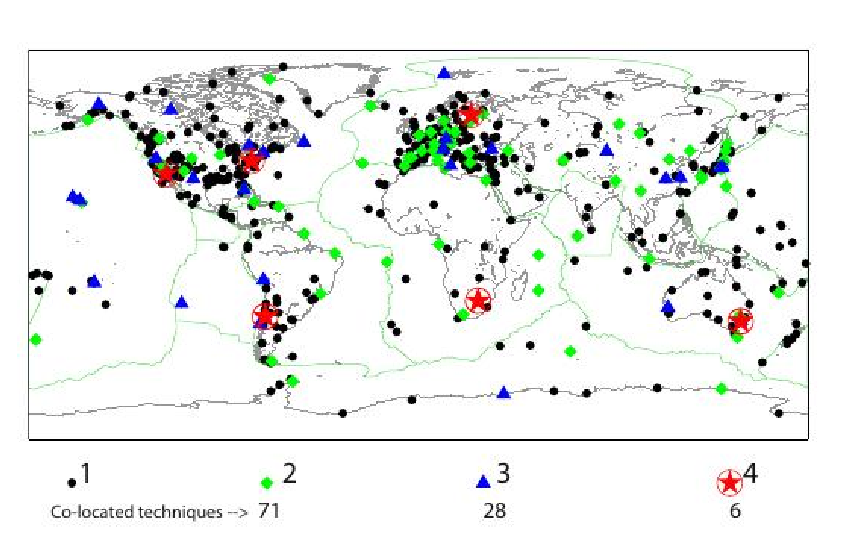
\includegraphics[scale=0.7]{ch2_ITRF_2008.eps}
\caption{\textit{Sieć stacji referencyjnych tworząca układ ITRF2008} źródło: \cite[][strona 38]{IERS_2010}}
\label{fig:ch2_itrf_2008}
\end{figure}
Układ ITRF składa się z współrzędnych oraz prędkości wybranych stacji referencyjnych oraz ich macierzy kowariancji. Parametry te są wyznaczane 
w centrach obliczeniowych Międzynarodowej Służby Ruchu Obrotowego Ziemi oraz Systemów Odniesienia (IERS) i publikowane w IERS Conventions. \cite[][strona 167]{ROCZNIK_2014}.
Warto jeszcze raz podkreślić, że dokładność wszystkich produktów służby IGS (International GNSS Service) takich jak orbity satelitów jest determinowana 
przez dokładność układu odniesienia do jakiego są one transformowane ( z układu niebieskiego ICRF) i następnie publikowane. Dokładność produktów IGS 
ma bezpośredni wpływ na wynik rozwiązania pozycji podczas nawigacji w czasie rzeczywistym.
Układ odniesienia IGS jest determinowany na podstawie tylko obserwacji GNSS wykonywanych na starannie wyselekcjonowanym podzbiorze 
stacjach referencyjnych IERS, i wpasowywany następnie za pomocą 14 parametrowej transformacji Helmerta do układu ITRF2008 \cite[]{ALTAMIMI_2009}.
Globalny układ odniesienia IGS jest zatem zgodny z układem ITRF2008. Ponadto wszystkie dane powstałe przed rokiem 2008 zostały odpowiednio 
przetransformowane w celu osiągnięcia jak największej wewnętrznej spójności \cite[][strona 15]{KOUBA_2009}.
Dla lepszego zrozumienia dalszych rozdziałów kluczowe wydaje się wyjaśnienie, że współrzędne stacji referencyjnych w układzie ITRF 
są wolne od wpływu pływów oceanicznych, pływów skorupy ziemskiej, oraz zmian położenia osi obrotu Ziemi (tzw. ruch bieguna).
W sensie globalnym pozycja każdej stacji referencyjnej podlega periodycznym fluktuacjom których amplituda jest rzędu kilku
decymetrów. W układzie ITRF powyższe wysokie częstotliwości są eliminowane za pomocą zastosowanych modeli. W pomiarach względnych o krótkich
bazach (<100km) fluktuacje są w przybliżeniu takie same, zatem do współrzędnych ITRF nie jest konieczne wprowadzanie poprawek.
Poprawki są jednak konieczne gdy wykonujemy pomiary w sensie absolutnym (aktualną pozycję wyznaczamy bezpośrednio względem znanych orbit)
w technice PPP lub w przypadku gdy pomiary różnicowe wykonywane są dla dużych odległości. \cite[][strona 11]{KOUBA_2009}
\section{Systemy GNSS}
	\subsection{GPS}
	\subsection{GLONASS}
	\subsection{GALILEO}
	\subsection{BaiDou-Compass}
	\subsection{Indian IRNSS}
\section{Algorytmy Pozycjonowania}
	\subsection{DGPS}
	\subsection{RTK}
	\subsection{PPP}
\section{Nawigacja Inercjalna}
\section{Zaawansowane metody opracowania obserwacji}

\noindent
Jeżeli wykorzystujemy w pomiarach pozycji DGPS – pomiar względny na podstawie pseudoodległości,
to dokładność lokalizacji pojazdu wynosi około 2m. 
Jeżeli natomiast zastosujemy technikę względnego opracowania obserwacji fazowych RTK dokładność wynosi 2cm.
Poniżej na rysunku \ref{fig:ch2_gpsReceiverExample} przedstawiono komputer z systemem wbudowanym,
który zintegrowano z odbiornikiem GPS \cite{CCTA_951_958}.
\begin{figure}[H]
\centering
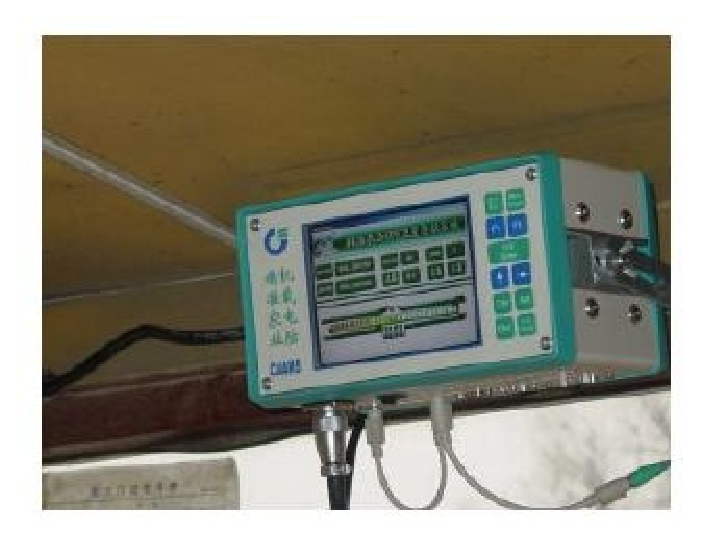
\includegraphics[scale=0.5]{ch2_gpsReceiverExample.eps}
\caption{\textit{Komputer z systemem wbudowanym, zintegrowanym z odbiornikiem GPS;} źródło: \cite[][strona 952]{CCTA_951_958}}
\label{fig:ch2_gpsReceiverExample}
\end{figure}
\noindent
%TODO trzeba opisać na czym polega filtracja Kalmana ( zaawansowane metody opracowania obserwacji)
